\documentclass{article}

\usepackage[utf8]{inputenc}
\usepackage{longtable}
\usepackage{authblk}
\usepackage{adjustbox}
\usepackage{natbib}



\title{LOS INDICES DE COLOMBIA}
% autores
\author[1]{\normalsize Sara Barón}
\affil[1]{\small  Escuela de Ingeniería,Universidad de los Andes\\
\texttt{{sj.baron10}@uniandes.edu.co}}


\date{29 de Junio de 2018}

\usepackage{Sweave}
\begin{document}
\Sconcordance{concordance:ProyectoFinal.tex:ProyectoFinal.Rnw:%
1 19 1 1 0 13 1 1 6 1 1 1 5 12 1 1 5 14 0 1 2 3 1 1 10 1 3 7 1 1 11 1 3 %
7 1 1 6 12 0 1 3 6 1 1 7 1 3 9 1 1 5 1 4 31 0 1 22 1 1 1 18 6 1 1 14 1 %
2 8 1}

\maketitle


\begin{abstract}
Este es mi primer trabajo en exploración y modelamiento de indices usando LATEX. Este trabajo lo he hecho bajo la filosofía de trabajo replicable. Este es mi primer trabajo en exploración y modelamiento de indices usando LATEX. Este trabajo lo he hecho bajo la filosofía de trabajo replicable. Este es mi primer trabajo en exploración y modelamiento de indices usando LATEX. Este trabajo lo he hecho bajo la filosofía de trabajo replicable. Este es mi primer trabajo en exploración y modelamiento de indices usando LATEX. Este trabajo lo he hecho bajo la filosofía de trabajo replicable.
\end{abstract}

\section*{Introducción}

Aquí les presento mi investigación sobre diversos indices sociales en el mundo. Los indices los conseguí de wikipedia, espero que les gusten mucho. Aquí les presento mi investigación sobre diversos indices sociales en el mundo. Los indices los conseguí de wikipedia, espero que les gusten mucho.Aquí les presento mi investigación sobre diversos indices sociales en el mundo. Los indices los conseguí de wikipedia, espero que les gusten mucho.Aqui les presento mi investigación sobre diversos indices sociales en el mundo. Los indices los conseguí de wikipedia, espero que les gusten mucho.
Aquí les presento mi investigacion sobre diversos indices sociales en el mundo. Los indices los conseguí de wikipedia, espero que les gusten mucho.Aqui les presento mi investigacion sobre diversos indices sociales en el mundo. Los indices los conseguí de wikipedia, espero que les gusten mucho.Aqui les presento mi investigacion sobre diversos indices sociales en el mundo. Los indices los conseguí de wikipedia, espero que les gusten mucho.





%Exploracion Univariada

Comencemos viendo que hay en la sección \ref{univariada} en la página \pageref{univariada}.

\clearpage

\section{Exploración Univariada}\label{univariada}

En esta sección exploro cada índice. En esta sección exploro cada índice. En esta sección exploro cada índice. En esta sección exploro cada ??ndice. En esta sección exploro cada índic. En esta sección exploro cada ??ndice. En esta sección exploro cada índice. En esta sección exploro cada índice. En esta sección exploro cada índice.

%Estad?sticos
% Table created by stargazer v.5.2.2 by Marek Hlavac, Harvard University. E-mail: hlavac at fas.harvard.edu
% Date and time: vie., jun. 29, 2018 - 7:22:25 p. m.
\begin{table}[!htbp] \centering 
  \caption{Medidas estad?sticas} 
  \label{stats} 
\begin{tabular}{@{\extracolsep{5pt}}lcc} 
\\[-1.8ex]\hline 
\hline \\[-1.8ex] 
Statistic & \multicolumn{1}{c}{N} & \multicolumn{1}{c}{Median} \\ 
\hline \\[-1.8ex] 
IDH & 32 & 0.804 \\ 
Población.Cabecera & 32 & 717,197 \\ 
Población.Resto & 32 & 268,111.5 \\ 
\hline \\[-1.8ex] 
\end{tabular} 
\end{table} 
\begin{figure}[h]
\centering
\begin{adjustbox}{width=7cm,height=7cm,clip,trim=1.5cm 0.5cm 0cm 1.5cm}
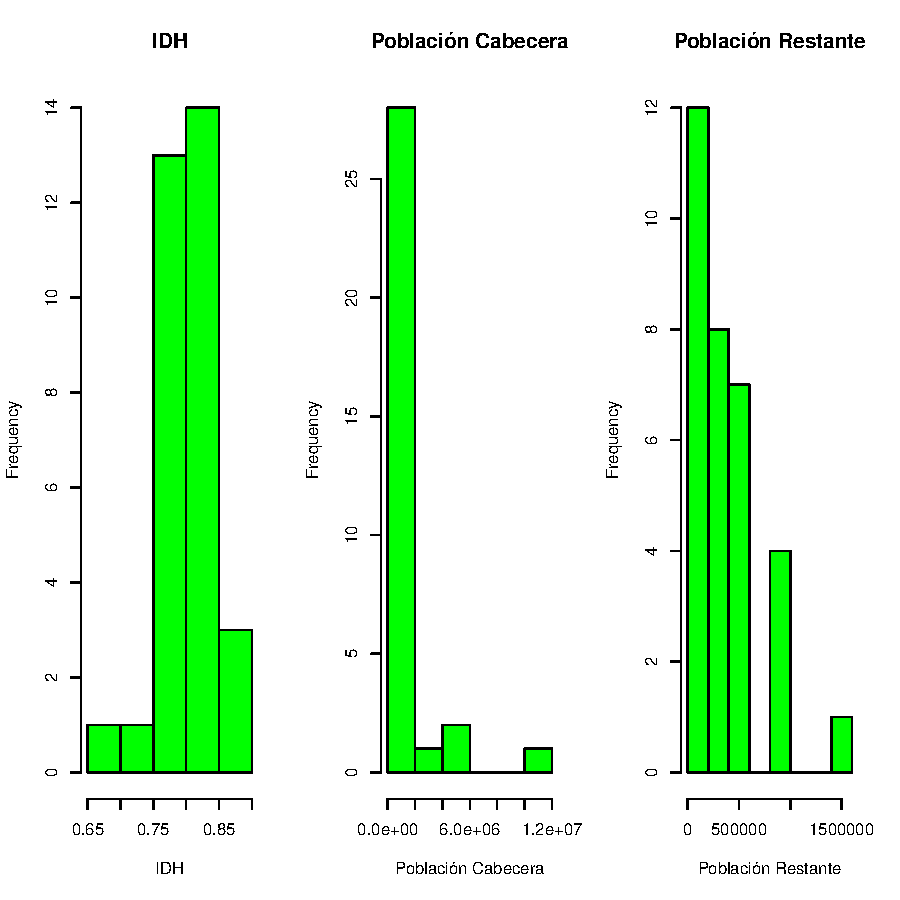
\includegraphics{ProyectoFinal-hist}
\end{adjustbox}
\caption{Histogramas}
\label{hist}
\end{figure}

\begin{figure}[h]
\centering
\begin{adjustbox}{width=7cm,height=7cm,clip,trim=1.5cm 0.5cm 0cm 1.5cm}
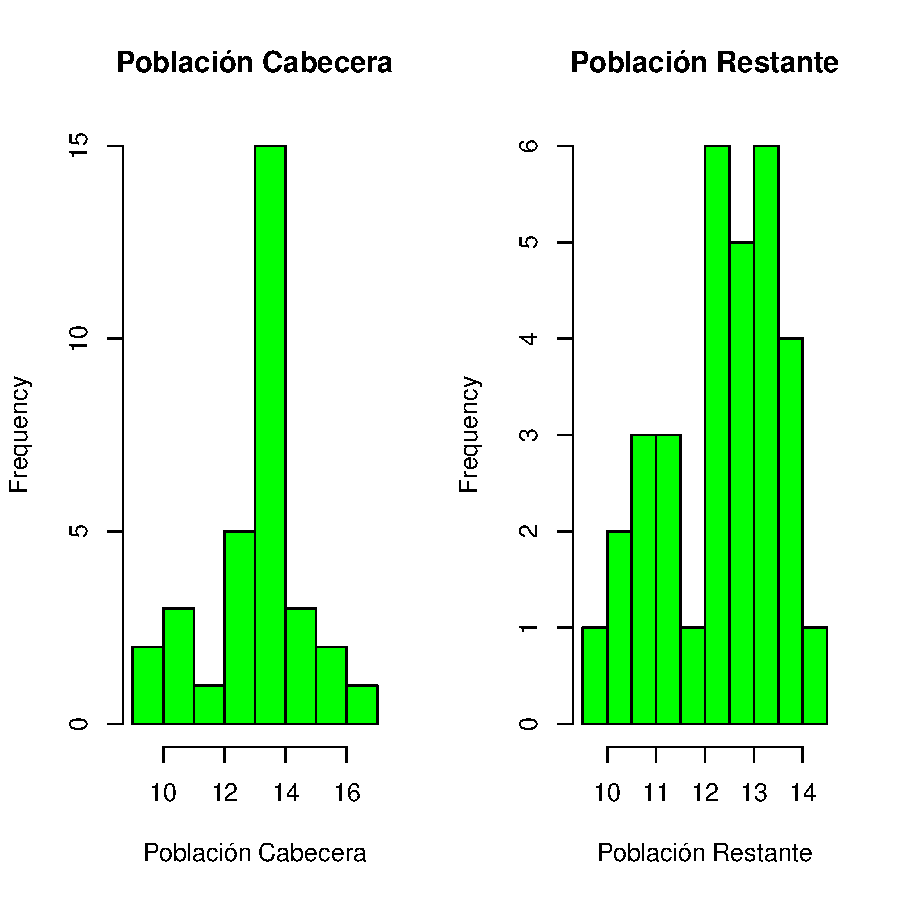
\includegraphics{ProyectoFinal-histnorm}
\end{adjustbox}
\caption{Histogramas Normalizados}
\label{histnorm}
\end{figure}


%Exploracion Bivariada ---------------------------------------------------

% Table created by stargazer v.5.2.2 by Marek Hlavac, Harvard University. E-mail: hlavac at fas.harvard.edu
% Date and time: vie., jun. 29, 2018 - 7:22:25 p. m.
\begin{table}[!htbp] \centering 
  \caption{Correlaci?n entre variables independientes} 
  \label{Corr} 
\begin{tabular}{@{\extracolsep{5pt}} cc} 
\\[-1.8ex]\hline 
\hline \\[-1.8ex] 
cabeLog & restoLog \\ 
\hline \\[-1.8ex] 
$0.487$ & $0.177$ \\ 
\hline \\[-1.8ex] 
\end{tabular} 
\end{table} 
% Correlaci?n entre variables independientes.

\begin{figure}[h]
\centering
\begin{adjustbox}{}

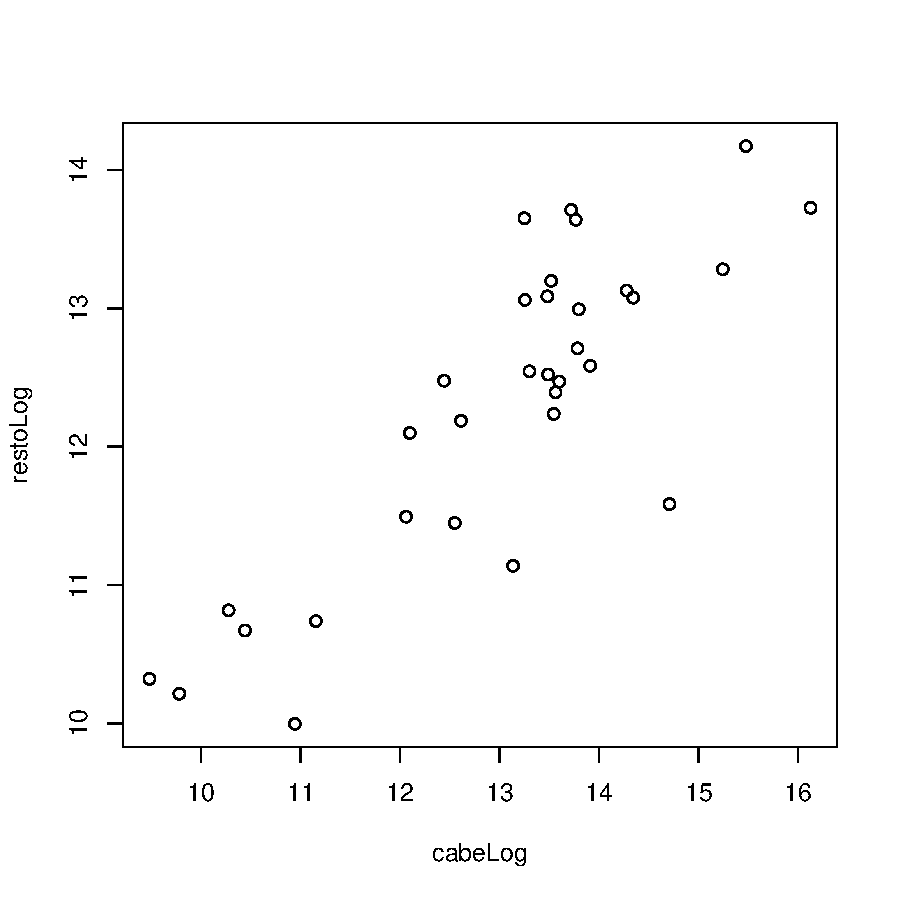
\includegraphics{ProyectoFinal-CorrInd}
\end{adjustbox}
\caption{Correlaci?n}
\label{CorrInd}
\end{figure}

%Modelos de Regresión ----------------------------------------------------

%Veamos los modelos propuestos. 
%Primero sin poblacion resto, luego con esa:


% Table created by stargazer v.5.2.2 by Marek Hlavac, Harvard University. E-mail: hlavac at fas.harvard.edu
% Date and time: vie., jun. 29, 2018 - 7:22:25 p. m.
\begin{table}[!htbp] \centering 
  \caption{Modelos de Regresi?n} 
  \label{regresiones} 
\begin{tabular}{@{\extracolsep{5pt}}lcc} 
\\[-1.8ex]\hline 
\hline \\[-1.8ex] 
 & \multicolumn{2}{c}{\textit{Dependent variable:}} \\ 
\cline{2-3} 
\\[-1.8ex] & \multicolumn{2}{c}{IDH} \\ 
\\[-1.8ex] & (1) & (2)\\ 
\hline \\[-1.8ex] 
 cabeLog & 0.013$^{***}$ & 0.031$^{***}$ \\ 
  & (0.004) & (0.007) \\ 
  & & \\ 
 restoLog &  & $-$0.030$^{***}$ \\ 
  &  & (0.010) \\ 
  & & \\ 
 Constant & 0.634$^{***}$ & 0.766$^{***}$ \\ 
  & (0.055) & (0.065) \\ 
  & & \\ 
\hline \\[-1.8ex] 
Observations & 32 & 32 \\ 
R$^{2}$ & 0.238 & 0.425 \\ 
Adjusted R$^{2}$ & 0.212 & 0.385 \\ 
Residual Std. Error & 0.037 (df = 30) & 0.033 (df = 29) \\ 
F Statistic & 9.347$^{***}$ (df = 1; 30) & 10.706$^{***}$ (df = 2; 29) \\ 
\hline 
\hline \\[-1.8ex] 
\textit{Note:}  & \multicolumn{2}{r}{$^{*}$p$<$0.1; $^{**}$p$<$0.05; $^{***}$p$<$0.01} \\ 
\end{tabular} 
\end{table} 



hola \cite{macqueen_methods_nodate}
\begin{figure}[h]
\centering
\begin{adjustbox}{}

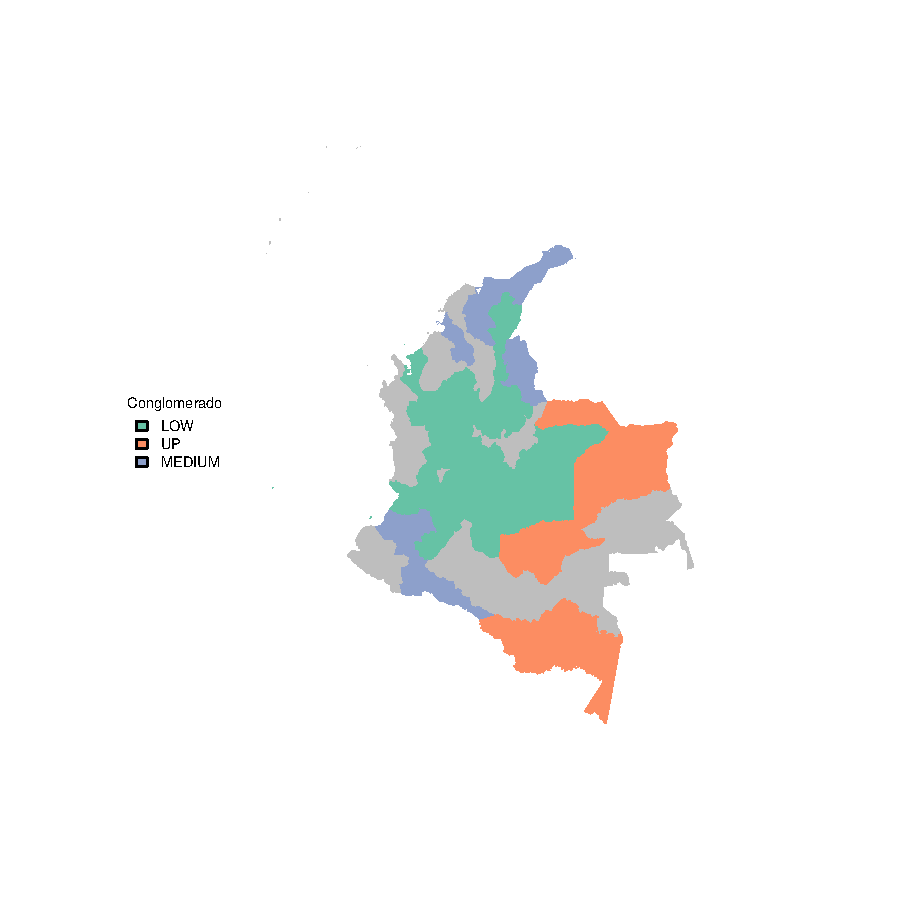
\includegraphics{ProyectoFinal-plotMapa}
\end{adjustbox}
\caption{Departamentos conglomerados seg?n sus indicadores}\label{clustmap}
\end{figure}

\bibliographystyle{abbrv}
\renewcommand{\refname}{Bibliografia}
\bibliography{colombia}

\end{document}
